\section{Results}
Both the monolithic network and the modular network were tested on the following test cases:
\begin{itemize}
\item 5 \times 5 grid world with the subnetworks evolving for 5, 10, 15, 50 generations and the overall network evolving for 100 generations in all cases. This was run for both ESP and NEAT
\item 10 \times 10 grid world with the subnetworks evolving for 5, 10, 15, 50 generations and the overall network evolving for 100 generations in all cases. This was also run for both ESP and NEAT
\item For the case of ESP, the algorithm was run with prey and hunter move probability set to 01, 0.5, 0.7 and 0.8. The number of generations of the sub-network evolution was fixed at 10. The overall network was run for 100 generations. 
\end{itemize}

First the experiments were run using NEAT.
Figure \ref{fig:MeanMAPNDCGPI1} a and b show the average predator fitness and the percentage improvement over the monolithic network for the 5x5 grid for the monolithic network, and for the case where the subnetwork was evolved for 50 generations. In this case the monolithic network seems to perform better than the modular network throughout. This might be because of the small size of the environment, which makes it easier for the monolithic network to learn, without having to contend with having to coordinate between the subnetworks. 

Figure \ref{fig:MeanMAPNDCGPI2} show the average predator fitness and the percentage improvement over the monolithic network for the 5x5 grid for the monolithic network, and the cases where the subnetworks were evolved for 5, 10, 15 and 50 generations. Again, the monolithic network is consistently better than the modular networks, and the number of generations the subnetworks were evolved doesn't seem to have a significant effect on the performance, although evolving the subnetwork for 15 generations seems to perform slightly better.

Very similar results are obtained for the 10 \times 10 grid size. The monolithic network performs much better in the case where the subnetwork is evolved for 50 generations (Figure \ref{fig:MeanMAPNDCGPI3}) and for cases where the subnetwork is evolved for 5, 10, 15 and 50 generations (Figure \ref{fig:MeanMAPNDCGPI4}).  
%%%%%%%%%%%%%%%%%%%%%%%%%%%%%%%%%%%%
%%%%%% AVERAGE 
%%%%%%%%%%%%%%%%%%%%%%%%%%%%%%%%%%%%
% Average % 5x5 % monolithic and 50
\begin{figure*}
\centering
\subfigure[5x5 Average Fitness]{
  \label{fig:neat_5x5_av_m50}
  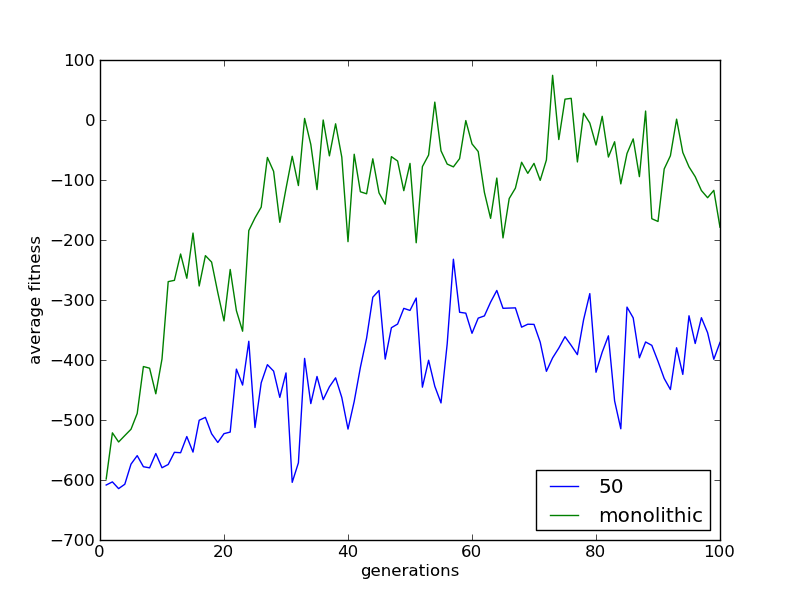
\includegraphics[scale=0.50]{figs/neat/average/5x5/monolithic_and_50/fitness-vs-generations.png}}
\hspace{1in}
\subfigure[5x5 Percent Improvement]{
  \label{fig:neat_5x5_av_m50_pi}
  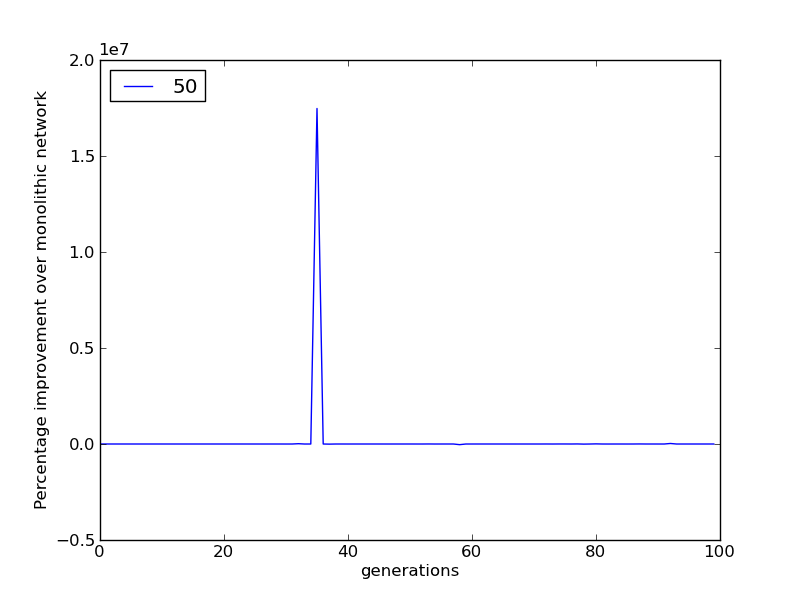
\includegraphics[scale=0.50]{figs/neat/average/5x5/monolithic_and_50/improvement-vs-generations.png}}
  \caption{Average fitness plotted over generations for a 5x5 grid for
  monolithic network and network seeded with modular networks evolved for 50
  generations}
  \label{fig:MeanMAPNDCGPI} % label for entire figure
\end{figure*}

% Average % 5x5 % all 
\begin{figure*}
\centering
\subfigure[5x5 Average Fitness]{
  \label{fig:neat_5x5_av_all}
  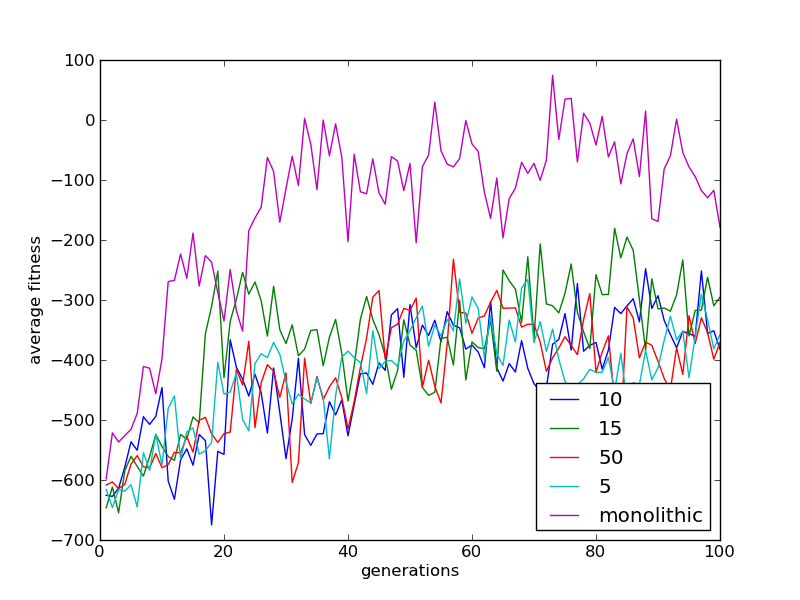
\includegraphics[scale=0.50]{figs/neat/average/5x5/all/fitness-vs-generations.png}}
\hspace{1in}
\subfigure[5x5 Percent Improvement]{
  \label{fig:neat_5x5_av_all_pi}
  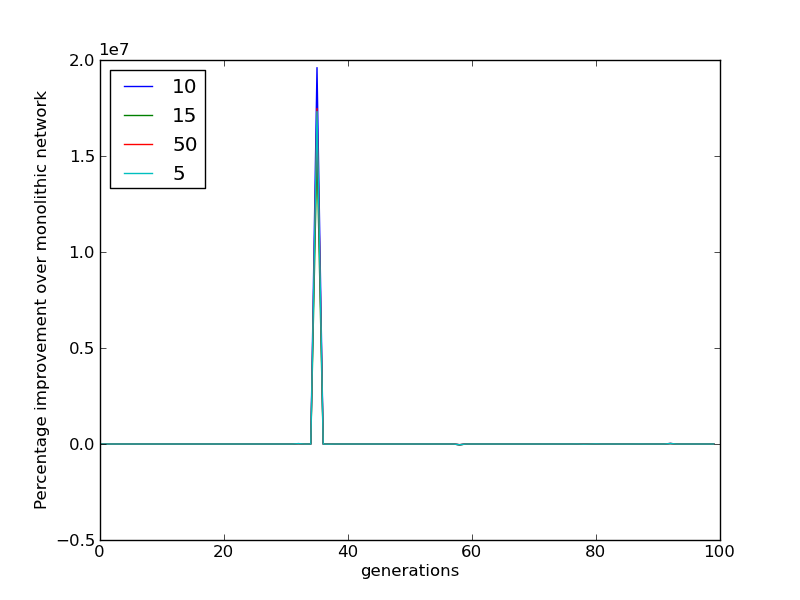
\includegraphics[scale=0.50]{figs/neat/average/5x5/all/improvement-vs-generations.png}}
  \caption{Average fitness plotted over generations for a 5x5 grid for
  monolithic network and network seeded with modular networks evolved for 5,
  10, 15 and 50 generations}
  \label{fig:MeanMAPNDCGPI} % label for entire figure
\end{figure*}

% Average % 10x10 % monolithic and 50
\begin{figure*}
\centering
\subfigure[10x10 Average Fitness]{
  \label{fig:neat_10x10_av_m50}
  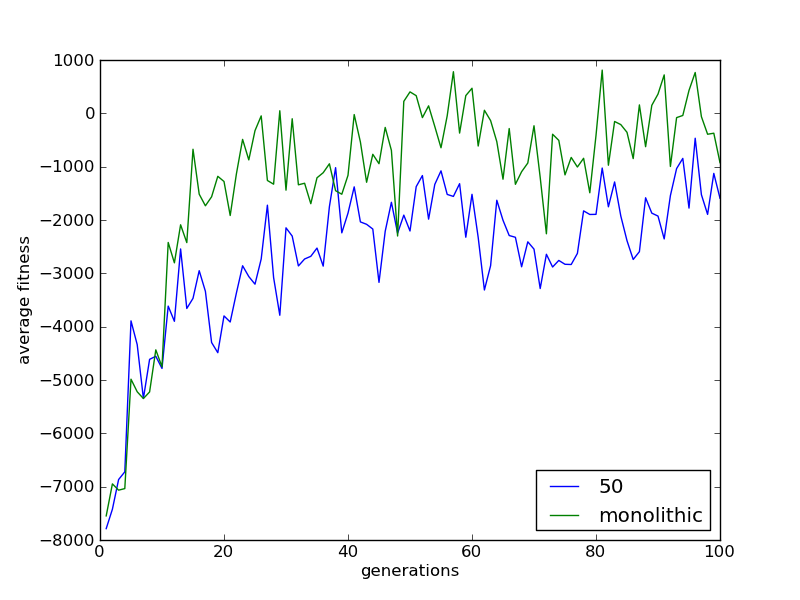
\includegraphics[scale=0.50]{figs/neat/average/10x10/monolithic_and_50/fitness-vs-generations.png}}
\hspace{1in}
\subfigure[10x10 Percent Improvement]{
  \label{fig:neat_10x10_av_m50_pi}
  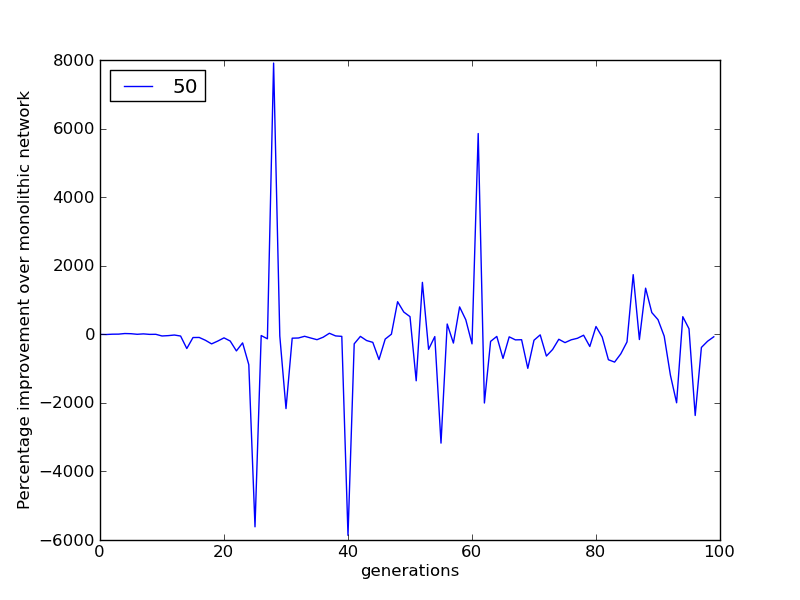
\includegraphics[scale=0.50]{figs/neat/average/10x10/monolithic_and_50/improvement-vs-generations.png}}
  \caption{Average fitness plotted over generations for a 10x10 grid for
  monolithic network and network seeded with modular networks evolved for 50
  generations}
  \label{fig:MeanMAPNDCGPI} % label for entire figure
\end{figure*}

% Average % 10x10 % all 
\begin{figure*}
\centering
\subfigure[10x10 Average Fitness]{
  \label{fig:neat_10x10_av_all}
  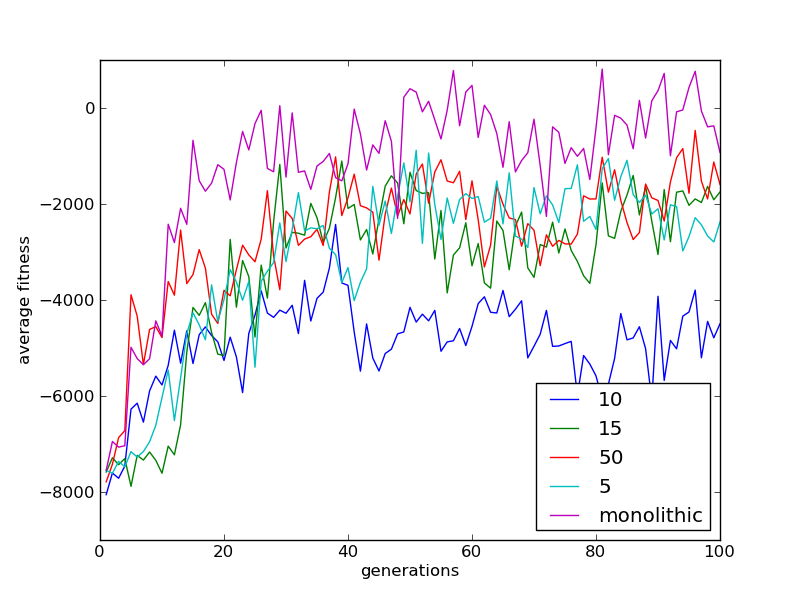
\includegraphics[scale=0.50]{figs/neat/average/10x10/all/fitness-vs-generations.png}}
\hspace{1in}
\subfigure[10x10 Percent Improvement]{
  \label{fig:neat_10x10_av_all_pi}
  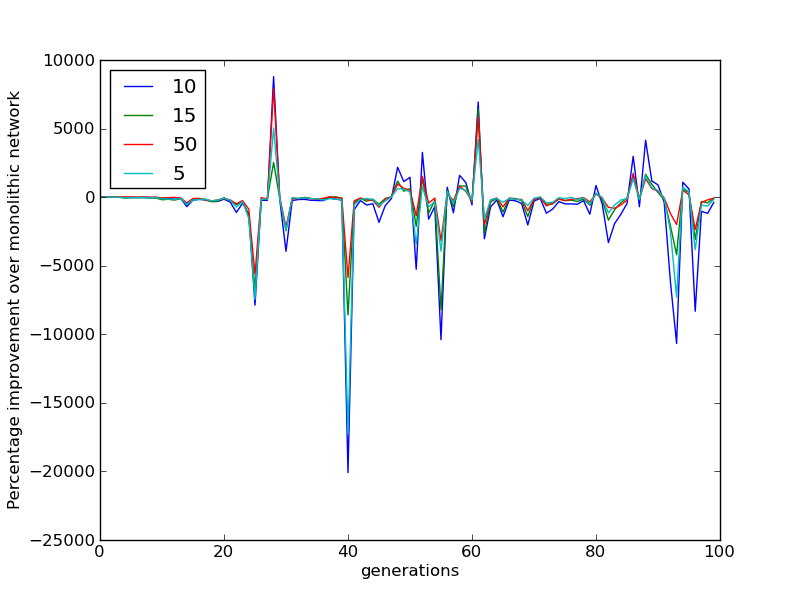
\includegraphics[scale=0.50]{figs/neat/average/10x10/all/improvement-vs-generations.png}}
  \caption{Average fitness plotted over generations for a 10x10 grid for
  monolithic network and network seeded with modular networks evolved for 5,
  10, 15 and 50 generations}
  \label{fig:MeanMAPNDCGPI} % label for entire figure
\end{figure*}

%%%%%%%%%%%%%%%%%%%%%%%%%%%%%%%%%%%%
%%%%%% CHAMPION
%%%%%%%%%%%%%%%%%%%%%%%%%%%%%%%%%%%%
% Champion % 5x5 % monolithic and 50
\begin{figure*}
\centering
\subfigure[5x5 Champion Fitness]{
  \label{fig:neat_5x5_c_m50}
  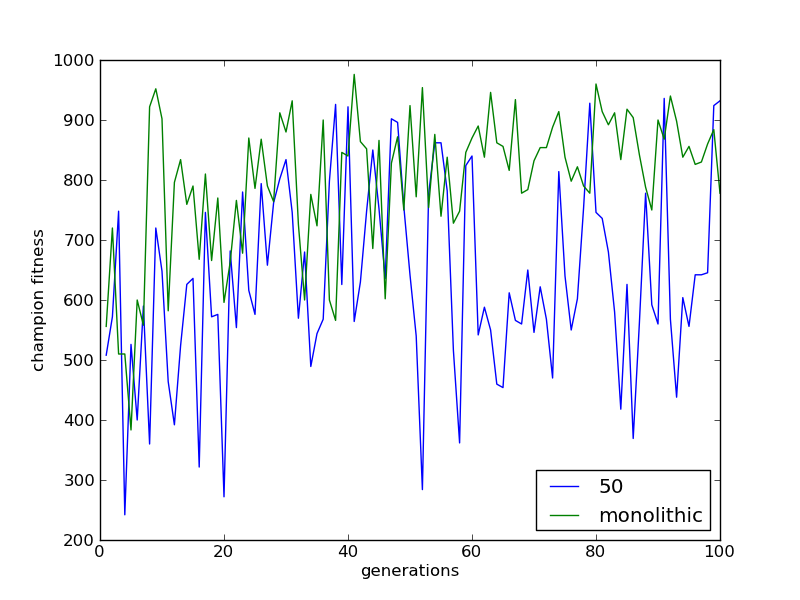
\includegraphics[scale=0.50]{figs/neat/champion/5x5/monolithic_and_50/fitness-vs-generations.png}}
\hspace{1in}
\subfigure[5x5 Percent Improvement]{
  \label{fig:neat_5x5_c_m50_pi}
  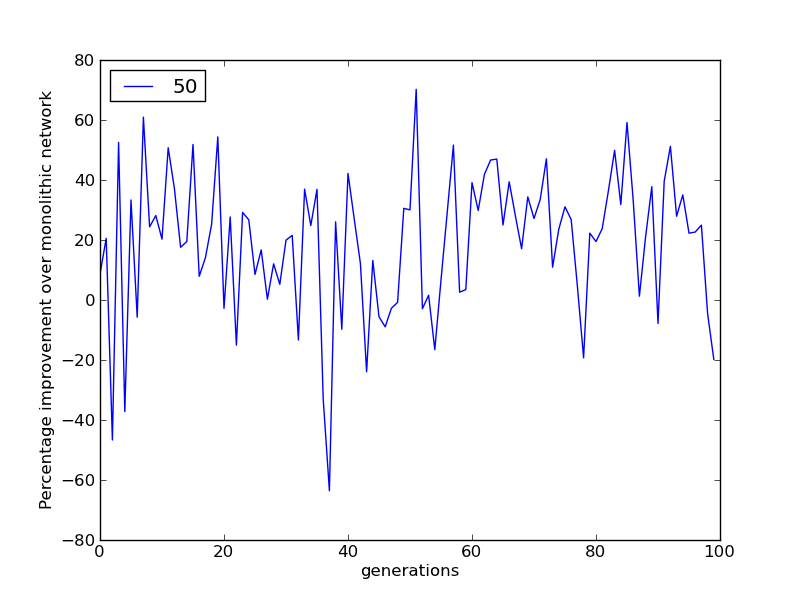
\includegraphics[scale=0.50]{figs/neat/champion/5x5/monolithic_and_50/improvement-vs-generations.png}}
  \caption{Champion fitness plotted over generations for a 5x5 grid for
  monolithic network and network seeded with modular networks evolved for 50
  generations}
  \label{fig:MeanMAPNDCGPI} % label for entire figure
\end{figure*}

% Champion % 5x5 % all 
\begin{figure*}
\centering
\subfigure[5x5 Champion Fitness]{
  \label{fig:neat_5x5_c_all}
  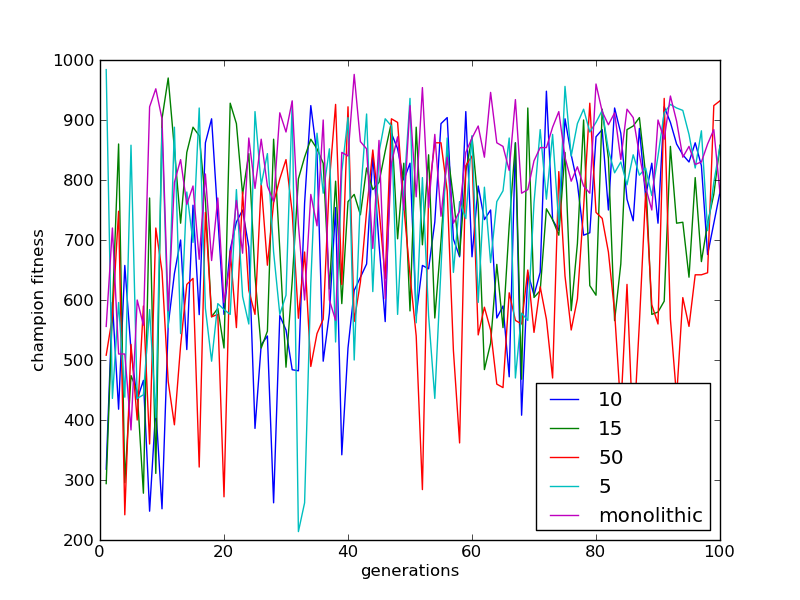
\includegraphics[scale=0.50]{figs/neat/champion/5x5/all/fitness-vs-generations.png}}
\hspace{1in}
\subfigure[5x5 Percent Improvement]{
  \label{fig:neat_5x5_c_all_pi}
  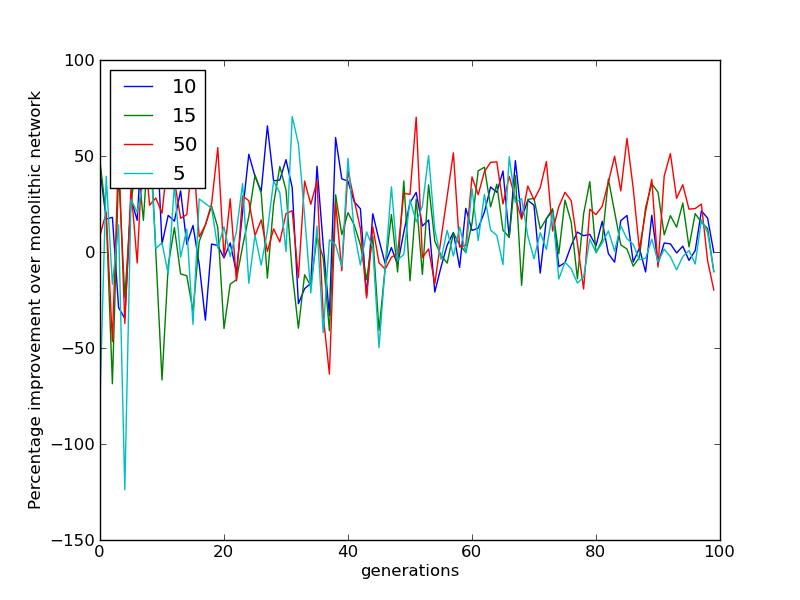
\includegraphics[scale=0.50]{figs/neat/champion/5x5/all/improvement-vs-generations.png}}
  \caption{Champion fitness plotted over generations for a 5x5 grid for
  monolithic network and network seeded with modular networks evolved for 5,
  10, 15 and 50 generations}
  \label{fig:MeanMAPNDCGPI} % label for entire figure
\end{figure*}

% Champion % 10x10 % monolithic and 50
\begin{figure*}
\centering
\subfigure[10x10 Champion Fitness]{
  \label{fig:neat_10x10_c_m50}
  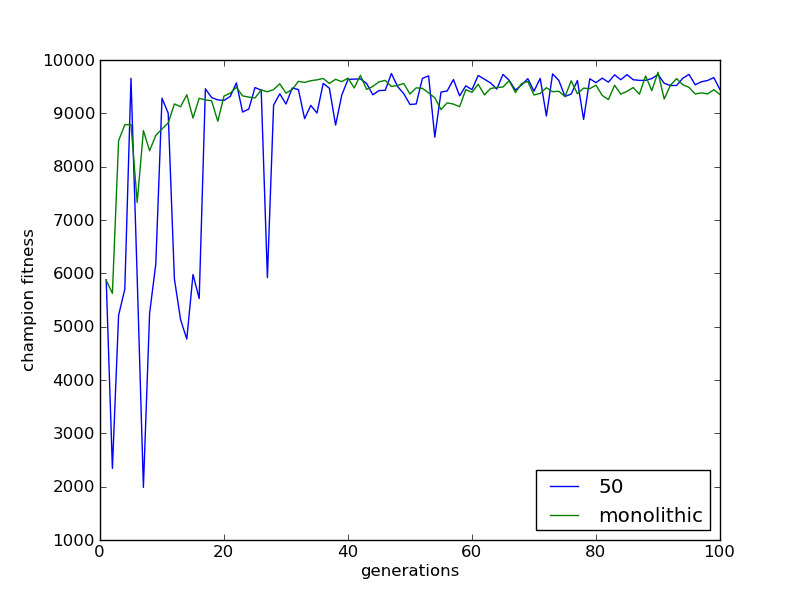
\includegraphics[scale=0.50]{figs/neat/champion/10x10/monolithic_and_50/fitness-vs-generations.png}}
\hspace{1in}
\subfigure[10x10 Percent Improvement]{
  \label{fig:neat_10x10_c_m50_pi}
  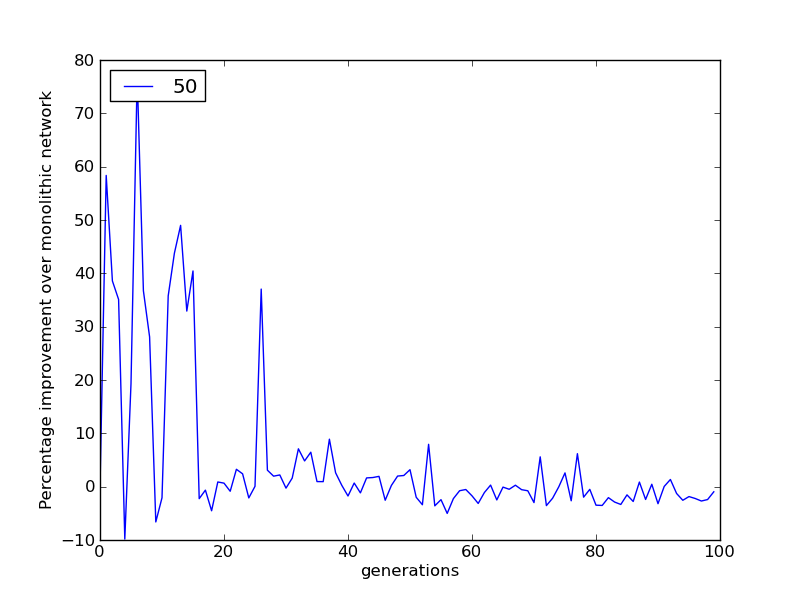
\includegraphics[scale=0.50]{figs/neat/champion/10x10/monolithic_and_50/improvement-vs-generations.png}}
  \caption{Champion fitness plotted over generations for a 10x10 grid for
  monolithic network and network seeded with modular networks evolved for 50
  generations}
  \label{fig:MeanMAPNDCGPI} % label for entire figure
\end{figure*}

% Champion % 10x10 % all 
\begin{figure*}
\centering
\subfigure[10x10 Champion Fitness]{
  \label{fig:neat_10x10_c_all}
  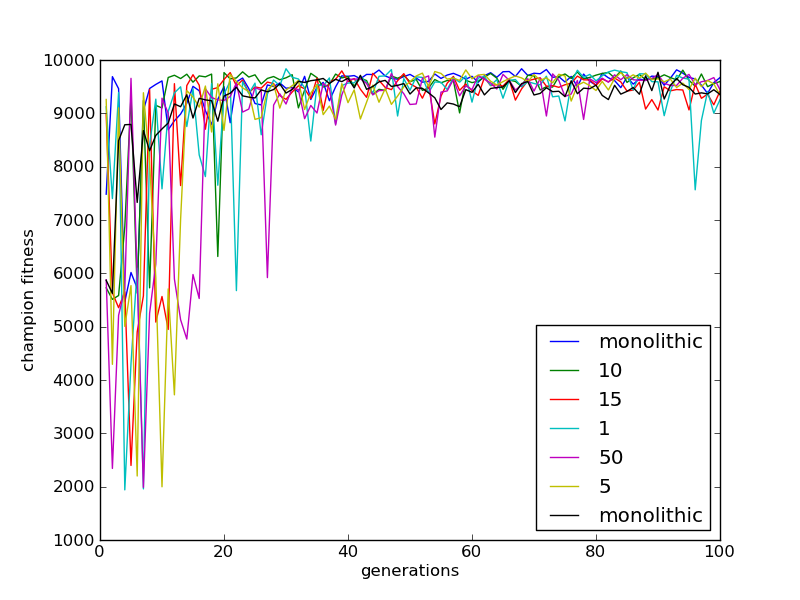
\includegraphics[scale=0.50]{figs/neat/champion/10x10/all/fitness-vs-generations.png}}
\hspace{1in}
\subfigure[10x10 Percent Improvement]{
  \label{fig:neat_10x10_c_all_pi}
  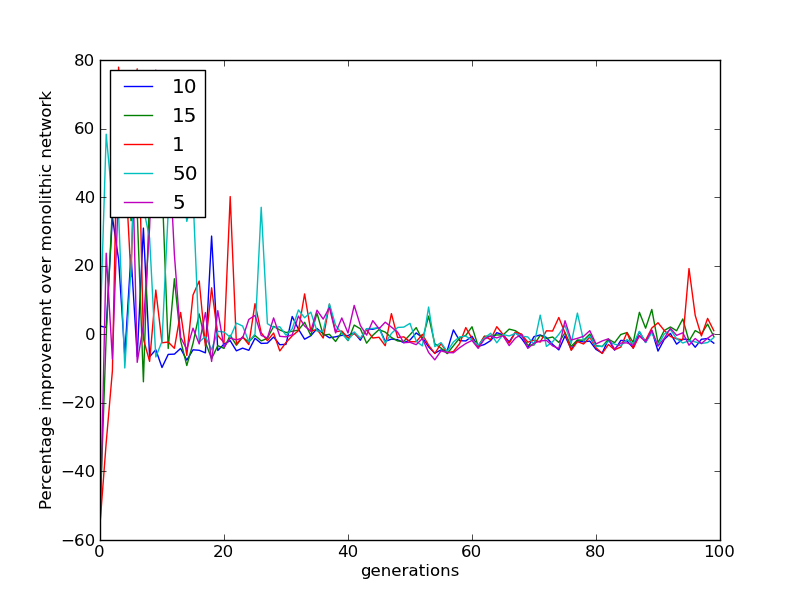
\includegraphics[scale=0.50]{figs/neat/champion/10x10/all/improvement-vs-generations.png}}
  \caption{Champion fitness plotted over generations for a 10x10 grid for
  monolithic network and network seeded with modular networks evolved for 5,
  10, 15 and 50 generations}
  \label{fig:MeanMAPNDCGPI} % label for entire figure
\end{figure*}

%%%%%%%%%%%%%%%%%%%%%%%%%%%%%%%%%%%%
%%%%%% AVERAGE 
%%%%%%%%%%%%%%%%%%%%%%%%%%%%%%%%%%%%
% Average % 5x5 % monolithic and all 
\begin{figure*}
\centering
\subfigure[5x5 Average Fitness]{
  \label{fig:esp_5x5_av_all}
  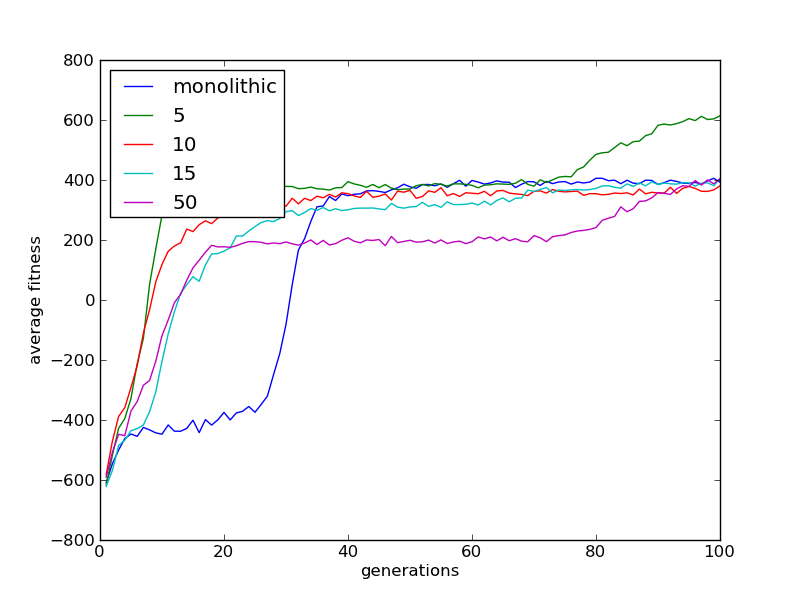
\includegraphics[scale=0.50]{figs/esp/fitness-vs-generations-5x5.png}}
\hspace{1in}
\subfigure[5x5 Percent Improvement]{
  \label{fig:esp_5x5_av_all_pi}
  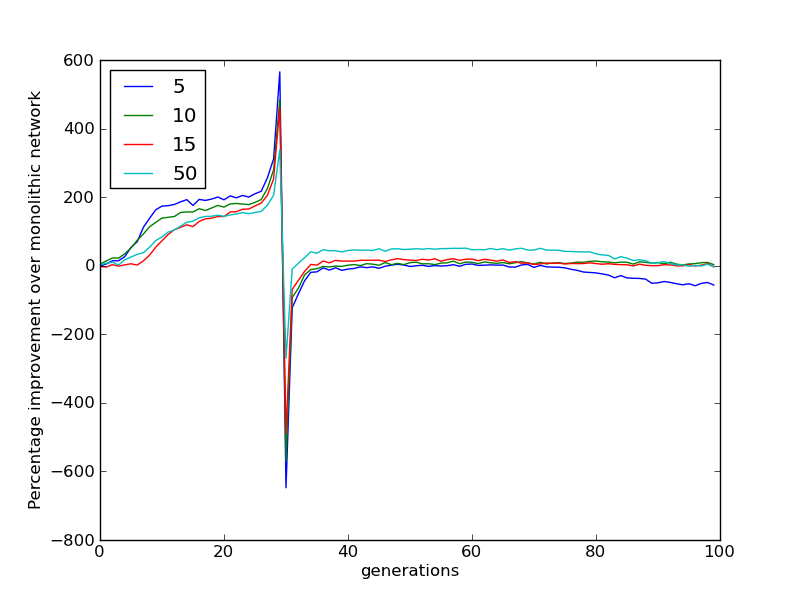
\includegraphics[scale=0.50]{figs/esp/improvement-vs-generations-5x5.png}}
  \caption{ESP: Average fitness plotted over generations for a 5x5 grid for
  monolithic network and network seeded with modular networks evolved for 5, 10, 15 and 50
  generations}
  \label{fig:MeanMAPNDCGPI9} % label for entire figure
\end{figure*}

% Average % 10x10 % monolithic and all 
\begin{figure*}
\centering
\subfigure[10x10 Average Fitness]{
  \label{fig:esp_10x10_av_all}
  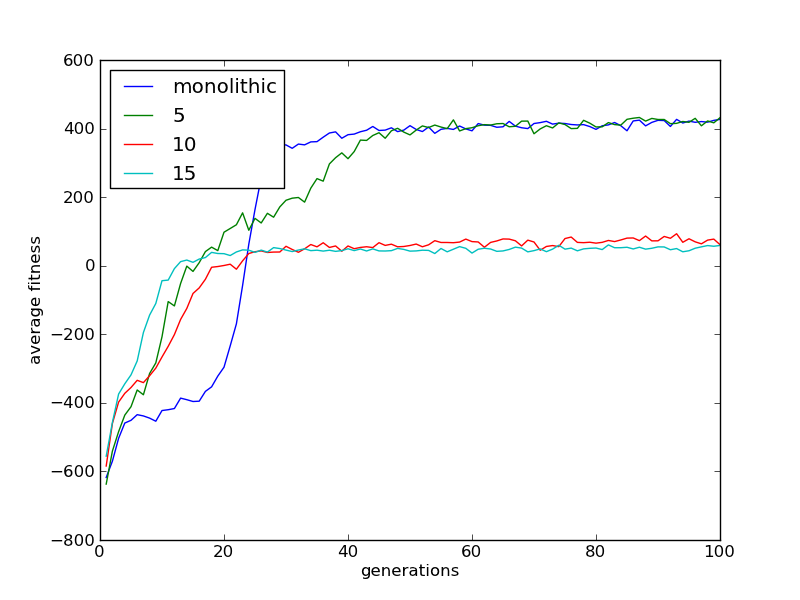
\includegraphics[scale=0.50]{figs/esp/fitness-vs-generations-10x10.png}}
\hspace{1in}
\subfigure[5x5 Percent Improvement]{
  \label{fig:esp_10x10_av_all_pi}
  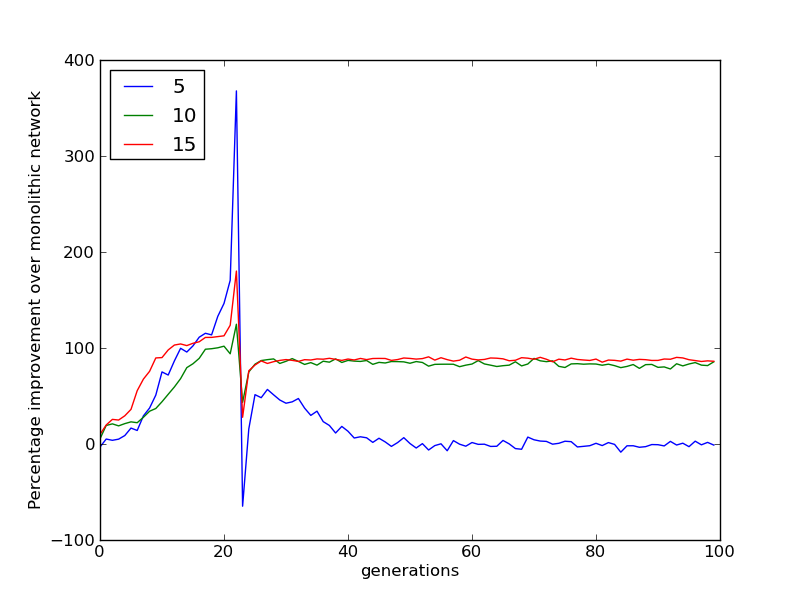
\includegraphics[scale=0.50]{figs/esp/improvement-vs-generations-10x10.png}}
  \caption{ESP: Average fitness plotted over generations for a 10x10 grid for
  monolithic network and network seeded with modular networks evolved for 5, 10, 15 and 50
  generations}
  \label{fig:MeanMAPNDCGPI10} % label for entire figure
\end{figure*}

% fitness-vs-generations-probs.png
\begin{figure*}[htp]
	\centering
	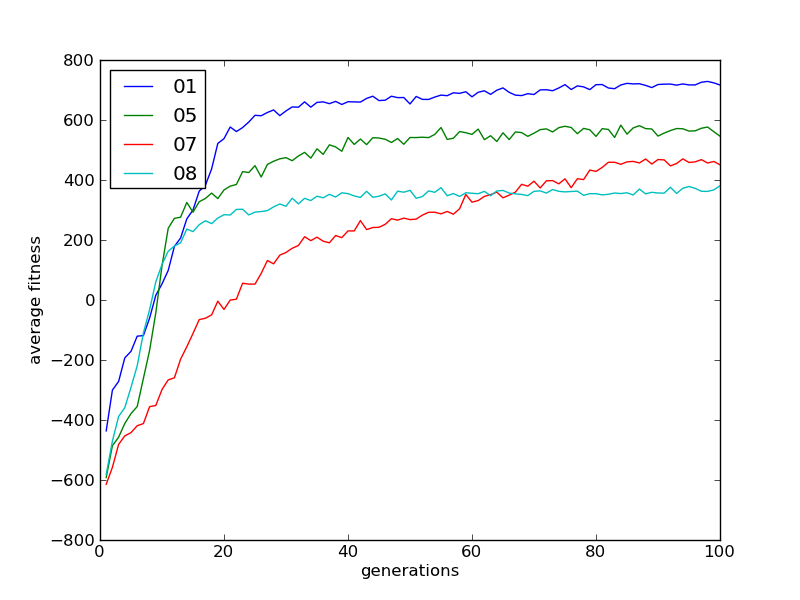
\includegraphics[scale=0.50]{figs/esp/fitness-vs-generations-probs.png}
	\caption{Performance of modular approach on a 5x5 grid with different move probabilities (0.1, 0.5, 0.7, 0,8) of hunter and prey (values for both are set to be the same)}
	\label{fig:MAPPIAll11}
\end{figure*}

